% Options for packages loaded elsewhere
\PassOptionsToPackage{unicode}{hyperref}
\PassOptionsToPackage{hyphens}{url}
\PassOptionsToPackage{dvipsnames,svgnames,x11names}{xcolor}
%
\documentclass[
  ignorenonframetext,
]{beamer}
\usepackage{pgfpages}
\setbeamertemplate{caption}[numbered]
\setbeamertemplate{caption label separator}{: }
\setbeamercolor{caption name}{fg=normal text.fg}
\beamertemplatenavigationsymbolsempty
% Prevent slide breaks in the middle of a paragraph
\widowpenalties 1 10000
\raggedbottom
\setbeamertemplate{part page}{
  \centering
  \begin{beamercolorbox}[sep=16pt,center]{part title}
    \usebeamerfont{part title}\insertpart\par
  \end{beamercolorbox}
}
\setbeamertemplate{section page}{
  \centering
  \begin{beamercolorbox}[sep=12pt,center]{part title}
    \usebeamerfont{section title}\insertsection\par
  \end{beamercolorbox}
}
\setbeamertemplate{subsection page}{
  \centering
  \begin{beamercolorbox}[sep=8pt,center]{part title}
    \usebeamerfont{subsection title}\insertsubsection\par
  \end{beamercolorbox}
}
\AtBeginPart{
  \frame{\partpage}
}
\AtBeginSection{
  \ifbibliography
  \else
    \frame{\sectionpage}
  \fi
}
\AtBeginSubsection{
  \frame{\subsectionpage}
}
\usepackage{amsmath,amssymb}
\usepackage{lmodern}
\usepackage{iftex}
\ifPDFTeX
  \usepackage[T1]{fontenc}
  \usepackage[utf8]{inputenc}
  \usepackage{textcomp} % provide euro and other symbols
\else % if luatex or xetex
  \usepackage{unicode-math}
  \defaultfontfeatures{Scale=MatchLowercase}
  \defaultfontfeatures[\rmfamily]{Ligatures=TeX,Scale=1}
\fi
% Use upquote if available, for straight quotes in verbatim environments
\IfFileExists{upquote.sty}{\usepackage{upquote}}{}
\IfFileExists{microtype.sty}{% use microtype if available
  \usepackage[]{microtype}
  \UseMicrotypeSet[protrusion]{basicmath} % disable protrusion for tt fonts
}{}
\makeatletter
\@ifundefined{KOMAClassName}{% if non-KOMA class
  \IfFileExists{parskip.sty}{%
    \usepackage{parskip}
  }{% else
    \setlength{\parindent}{0pt}
    \setlength{\parskip}{6pt plus 2pt minus 1pt}}
}{% if KOMA class
  \KOMAoptions{parskip=half}}
\makeatother
\usepackage{xcolor}
\newif\ifbibliography
\usepackage{color}
\usepackage{fancyvrb}
\newcommand{\VerbBar}{|}
\newcommand{\VERB}{\Verb[commandchars=\\\{\}]}
\DefineVerbatimEnvironment{Highlighting}{Verbatim}{commandchars=\\\{\}}
% Add ',fontsize=\small' for more characters per line
\usepackage{framed}
\definecolor{shadecolor}{RGB}{248,248,248}
\newenvironment{Shaded}{\begin{snugshade}}{\end{snugshade}}
\newcommand{\AlertTok}[1]{\textcolor[rgb]{0.94,0.16,0.16}{#1}}
\newcommand{\AnnotationTok}[1]{\textcolor[rgb]{0.56,0.35,0.01}{\textbf{\textit{#1}}}}
\newcommand{\AttributeTok}[1]{\textcolor[rgb]{0.77,0.63,0.00}{#1}}
\newcommand{\BaseNTok}[1]{\textcolor[rgb]{0.00,0.00,0.81}{#1}}
\newcommand{\BuiltInTok}[1]{#1}
\newcommand{\CharTok}[1]{\textcolor[rgb]{0.31,0.60,0.02}{#1}}
\newcommand{\CommentTok}[1]{\textcolor[rgb]{0.56,0.35,0.01}{\textit{#1}}}
\newcommand{\CommentVarTok}[1]{\textcolor[rgb]{0.56,0.35,0.01}{\textbf{\textit{#1}}}}
\newcommand{\ConstantTok}[1]{\textcolor[rgb]{0.00,0.00,0.00}{#1}}
\newcommand{\ControlFlowTok}[1]{\textcolor[rgb]{0.13,0.29,0.53}{\textbf{#1}}}
\newcommand{\DataTypeTok}[1]{\textcolor[rgb]{0.13,0.29,0.53}{#1}}
\newcommand{\DecValTok}[1]{\textcolor[rgb]{0.00,0.00,0.81}{#1}}
\newcommand{\DocumentationTok}[1]{\textcolor[rgb]{0.56,0.35,0.01}{\textbf{\textit{#1}}}}
\newcommand{\ErrorTok}[1]{\textcolor[rgb]{0.64,0.00,0.00}{\textbf{#1}}}
\newcommand{\ExtensionTok}[1]{#1}
\newcommand{\FloatTok}[1]{\textcolor[rgb]{0.00,0.00,0.81}{#1}}
\newcommand{\FunctionTok}[1]{\textcolor[rgb]{0.00,0.00,0.00}{#1}}
\newcommand{\ImportTok}[1]{#1}
\newcommand{\InformationTok}[1]{\textcolor[rgb]{0.56,0.35,0.01}{\textbf{\textit{#1}}}}
\newcommand{\KeywordTok}[1]{\textcolor[rgb]{0.13,0.29,0.53}{\textbf{#1}}}
\newcommand{\NormalTok}[1]{#1}
\newcommand{\OperatorTok}[1]{\textcolor[rgb]{0.81,0.36,0.00}{\textbf{#1}}}
\newcommand{\OtherTok}[1]{\textcolor[rgb]{0.56,0.35,0.01}{#1}}
\newcommand{\PreprocessorTok}[1]{\textcolor[rgb]{0.56,0.35,0.01}{\textit{#1}}}
\newcommand{\RegionMarkerTok}[1]{#1}
\newcommand{\SpecialCharTok}[1]{\textcolor[rgb]{0.00,0.00,0.00}{#1}}
\newcommand{\SpecialStringTok}[1]{\textcolor[rgb]{0.31,0.60,0.02}{#1}}
\newcommand{\StringTok}[1]{\textcolor[rgb]{0.31,0.60,0.02}{#1}}
\newcommand{\VariableTok}[1]{\textcolor[rgb]{0.00,0.00,0.00}{#1}}
\newcommand{\VerbatimStringTok}[1]{\textcolor[rgb]{0.31,0.60,0.02}{#1}}
\newcommand{\WarningTok}[1]{\textcolor[rgb]{0.56,0.35,0.01}{\textbf{\textit{#1}}}}
\usepackage{graphicx}
\makeatletter
\def\maxwidth{\ifdim\Gin@nat@width>\linewidth\linewidth\else\Gin@nat@width\fi}
\def\maxheight{\ifdim\Gin@nat@height>\textheight\textheight\else\Gin@nat@height\fi}
\makeatother
% Scale images if necessary, so that they will not overflow the page
% margins by default, and it is still possible to overwrite the defaults
% using explicit options in \includegraphics[width, height, ...]{}
\setkeys{Gin}{width=\maxwidth,height=\maxheight,keepaspectratio}
% Set default figure placement to htbp
\makeatletter
\def\fps@figure{htbp}
\makeatother
\setlength{\emergencystretch}{3em} % prevent overfull lines
\providecommand{\tightlist}{%
  \setlength{\itemsep}{0pt}\setlength{\parskip}{0pt}}
\setcounter{secnumdepth}{-\maxdimen} % remove section numbering
\newlength{\cslhangindent}
\setlength{\cslhangindent}{1.5em}
\newlength{\csllabelwidth}
\setlength{\csllabelwidth}{3em}
\newlength{\cslentryspacingunit} % times entry-spacing
\setlength{\cslentryspacingunit}{\parskip}
\newenvironment{CSLReferences}[2] % #1 hanging-ident, #2 entry spacing
 {% don't indent paragraphs
  \setlength{\parindent}{0pt}
  % turn on hanging indent if param 1 is 1
  \ifodd #1
  \let\oldpar\par
  \def\par{\hangindent=\cslhangindent\oldpar}
  \fi
  % set entry spacing
  \setlength{\parskip}{#2\cslentryspacingunit}
 }%
 {}
\usepackage{calc}
\newcommand{\CSLBlock}[1]{#1\hfill\break}
\newcommand{\CSLLeftMargin}[1]{\parbox[t]{\csllabelwidth}{#1}}
\newcommand{\CSLRightInline}[1]{\parbox[t]{\linewidth - \csllabelwidth}{#1}\break}
\newcommand{\CSLIndent}[1]{\hspace{\cslhangindent}#1}
\usepackage{graphicx}
\usepackage{bm}
\definecolor{foreground}{RGB}{255,255,255}
\definecolor{background}{RGB}{34,28,54}
\definecolor{title}{RGB}{105,165,255}
\definecolor{gray}{RGB}{175,175,175}
\definecolor{lightgray}{RGB}{225,225,225}
\definecolor{subtitle}{RGB}{232,234,255}
\definecolor{hilight}{RGB}{112,224,255}
\definecolor{vhilight}{RGB}{255,111,207}
\setbeamertemplate{footline}[page number]
\ifLuaTeX
  \usepackage{selnolig}  % disable illegal ligatures
\fi
\IfFileExists{bookmark.sty}{\usepackage{bookmark}}{\usepackage{hyperref}}
\IfFileExists{xurl.sty}{\usepackage{xurl}}{} % add URL line breaks if available
\urlstyle{same} % disable monospaced font for URLs
\hypersetup{
  pdftitle={STAT 528 - Advanced Regression Analysis II},
  pdfauthor={Generalized Linear Models Diagnostics},
  colorlinks=true,
  linkcolor={Maroon},
  filecolor={Maroon},
  citecolor={Blue},
  urlcolor={blue},
  pdfcreator={LaTeX via pandoc}}

\title{STAT 528 - Advanced Regression Analysis II}
\author{Generalized Linear Models Diagnostics}
\date{}
\institute{Daniel J. Eck (with credit to Lu Yang)\\
Department of Statistics\\
University of Illinois}

\begin{document}
\frame{\titlepage}

\begin{frame}{Learning Objectives Today}
\protect\hypertarget{learning-objectives-today}{}
\begin{itemize}
\tightlist
\item
  GLM diagnostics
\end{itemize}
\end{frame}

\begin{frame}{}
\protect\hypertarget{section}{}
\begin{itemize}
\tightlist
\item
  The diagnostic methods for GLMs mirror those used for Gaussian linear
  models.
\item
  However, some adaptations are necessary and, depending on the type of
  GLM, not all diagnostic methods will be applicable.
\end{itemize}
\end{frame}

\begin{frame}{Leverage and Influence}
\protect\hypertarget{leverage-and-influence}{}
\begin{itemize}
\tightlist
\item
  Hat matrix
  \[\mathbf{H}=\mathbf{W}^{1/2}\mathbf{X}(\mathbf{X}'\mathbf{W}\mathbf{X})^{-1}\mathbf{X}'\mathbf{W}^{1/2}\]
  where \(\mathbf{W} = diag(w)\) are weights in IRLS.
\item
  One important difference from the linear model case is that the
  leverages are no longer just a function of \(\mathbf{X}\) and now
  depend on the response through the weights \(\mathbf{W}\)
\item
  Cook's distance
  \[D_i=\frac{(\hat{\bm\beta}_{(i)}-\hat{\bm\beta})'(\mathbf{X}'\mathbf{W}\mathbf{X})(\hat{\bm\beta}_{(i)}-\hat{\bm\beta})}{p'\hat{\phi}}\]
\end{itemize}
\end{frame}

\begin{frame}[fragile]{Galapagos data: large mean discrete outcomes}
\protect\hypertarget{galapagos-data-large-mean-discrete-outcomes}{}
\begin{itemize}
\tightlist
\item
  There are 30 Galapagos islands and 7 variables in the data set. The
  relationship between the number of plant species and several
  geographic variables is of interest.
\end{itemize}

\scriptsize

\begin{Shaded}
\begin{Highlighting}[]
\FunctionTok{data}\NormalTok{(gala, }\AttributeTok{package=}\StringTok{"faraway"}\NormalTok{)}
\FunctionTok{head}\NormalTok{(gala)}
\end{Highlighting}
\end{Shaded}

\begin{verbatim}
##              Species Endemics  Area Elevation Nearest Scruz Adjacent
## Baltra            58       23 25.09       346     0.6   0.6     1.84
## Bartolome         31       21  1.24       109     0.6  26.3   572.33
## Caldwell           3        3  0.21       114     2.8  58.7     0.78
## Champion          25        9  0.10        46     1.9  47.4     0.18
## Coamano            2        1  0.05        77     1.9   1.9   903.82
## Daphne.Major      18       11  0.34       119     8.0   8.0     1.84
\end{verbatim}

\begin{Shaded}
\begin{Highlighting}[]
\NormalTok{modp }\OtherTok{\textless{}{-}} \FunctionTok{glm}\NormalTok{(Species }\SpecialCharTok{\textasciitilde{}}\NormalTok{ .,}\AttributeTok{family=}\NormalTok{poisson,gala)}
\end{Highlighting}
\end{Shaded}
\end{frame}

\begin{frame}[fragile]{}
\protect\hypertarget{section-1}{}
\scriptsize

\begin{Shaded}
\begin{Highlighting}[]
\FunctionTok{par}\NormalTok{(}\AttributeTok{mfrow=}\FunctionTok{c}\NormalTok{(}\DecValTok{1}\NormalTok{,}\DecValTok{2}\NormalTok{))}
\FunctionTok{plot}\NormalTok{(modp,}\AttributeTok{which=}\DecValTok{4}\NormalTok{)}
\FunctionTok{plot}\NormalTok{(modp,}\AttributeTok{which=}\DecValTok{5}\NormalTok{)}
\end{Highlighting}
\end{Shaded}

\includegraphics{week8_p1_files/figure-beamer/unnamed-chunk-2-1.pdf}
\end{frame}

\begin{frame}{Residuals}
\protect\hypertarget{residuals}{}
\begin{itemize}
\tightlist
\item
  Pearson residuals
  \[\hat{e}_{Pi}=\frac{y_i-\hat{\mu}_i}{\sqrt{V(\hat{\mu}_i)}}\]
\item
  \(X^2=\sum_i\hat{e}_{Pi}\)
\item
  Let deviance \(D=\sum_id_i\), deviance
  residuals\[\hat{e}_{Di}=\mathrm{sign}\left(y_i-\hat{\mu}_i\right)\sqrt{d_i}\]
\item
  \(D=\sum_{i=1}^n\hat{e}_{Di}^2\)
\end{itemize}
\end{frame}

\begin{frame}[fragile]{}
\protect\hypertarget{section-2}{}
\scriptsize

\begin{Shaded}
\begin{Highlighting}[]
\FunctionTok{plot}\NormalTok{(}\FunctionTok{residuals}\NormalTok{(modp,}\AttributeTok{type=}\StringTok{"deviance"}\NormalTok{) }\SpecialCharTok{\textasciitilde{}} \FunctionTok{predict}\NormalTok{(modp,}\AttributeTok{type=}\StringTok{"response"}\NormalTok{),}
\AttributeTok{xlab=}\FunctionTok{expression}\NormalTok{(}\FunctionTok{hat}\NormalTok{(mu)),}\AttributeTok{ylab=}\StringTok{"Deviance residuals"}\NormalTok{)}
\FunctionTok{abline}\NormalTok{(}\AttributeTok{h=}\DecValTok{0}\NormalTok{)}
\end{Highlighting}
\end{Shaded}

\includegraphics{week8_p1_files/figure-beamer/unnamed-chunk-3-1.pdf}
\end{frame}

\begin{frame}{Potential remedies}
\protect\hypertarget{potential-remedies}{}
\begin{itemize}
\tightlist
\item
  Is there any nonlinear relationship between the predicted values and
  the residuals?

  \begin{itemize}
  \tightlist
  \item
    A change link function
  \item
    A change in the choice of predictors or transformations on these
    predictors
  \end{itemize}
\item
  The assumptions of the GLM would require constant variance in the plot

  \begin{itemize}
  \tightlist
  \item
    A change in the variance function, quasi-likelihood GLM
  \end{itemize}
\end{itemize}
\end{frame}

\begin{frame}[fragile]{QQ plot}
\protect\hypertarget{qq-plot}{}
\scriptsize

\begin{Shaded}
\begin{Highlighting}[]
\FunctionTok{qqnorm}\NormalTok{(}\FunctionTok{residuals}\NormalTok{(modp,}\AttributeTok{type=}\StringTok{"deviance"}\NormalTok{))}
\FunctionTok{qqline}\NormalTok{(}\FunctionTok{residuals}\NormalTok{(modp,}\AttributeTok{type=}\StringTok{"deviance"}\NormalTok{))}
\end{Highlighting}
\end{Shaded}

\includegraphics{week8_p1_files/figure-beamer/unnamed-chunk-4-1.pdf}
\end{frame}

\begin{frame}[fragile]{Half-normal plots}
\protect\hypertarget{half-normal-plots}{}
\begin{itemize}
\tightlist
\item
  One can use a half-normal plot that compares the sorted absolute
  residuals and the quantiles of the half-normal distribution:
  \(\Phi^{-1}\left(\frac{n+i}{2n+1}\right)~i=1,\ldots,n\)
\item
  We seek outliers which may be identified as points off the trend
\end{itemize}

\scriptsize

\begin{Shaded}
\begin{Highlighting}[]
\FunctionTok{library}\NormalTok{(faraway)}
\FunctionTok{halfnorm}\NormalTok{(}\FunctionTok{residuals}\NormalTok{(modp))}
\end{Highlighting}
\end{Shaded}

\includegraphics{week8_p1_files/figure-beamer/unnamed-chunk-5-1.pdf}
\end{frame}

\begin{frame}[fragile]{Small mean discrete outcomes: LGPIF data}
\protect\hypertarget{small-mean-discrete-outcomes-lgpif-data}{}
\begin{itemize}
\tightlist
\item
  In some cases, plots of the residuals are not particularly helpful.
\item
  For a binary response, the residual can only take two possible values
  for given predicted response. This is the most extreme situation, but
  similar discreteness can occur for binomial responses with small group
  sizes and Poisson responses that are small.
\end{itemize}

\scriptsize

\begin{Shaded}
\begin{Highlighting}[]
\NormalTok{freqinBC }\OtherTok{\textless{}{-}} \FunctionTok{readRDS}\NormalTok{(}\StringTok{"freqinBC.rds"}\NormalTok{)}
\FunctionTok{table}\NormalTok{(freqinBC}\SpecialCharTok{$}\NormalTok{FreqBC)}
\end{Highlighting}
\end{Shaded}

\begin{verbatim}
## 
##    0    1    2    3    4    5    6    7    8    9   10   11   12   13   14   15 
## 3976  997  333  136   76   31   19   19   16    5    7    2    4    5    5    2 
##   16   17   18   20   22   23   24   33   34   53   55   65   78   86   89   97 
##    4    3    1    1    1    1    1    1    1    1    1    1    1    1    1    1 
##   98  108  133  154  201  231 
##    1    1    1    1    1    1
\end{verbatim}
\end{frame}

\begin{frame}[fragile]{}
\protect\hypertarget{section-3}{}
\scriptsize

\begin{Shaded}
\begin{Highlighting}[]
\CommentTok{\# Possion GLM}
\NormalTok{freqmodelBC }\OtherTok{\textless{}{-}} \FunctionTok{glm}\NormalTok{(FreqBC }\SpecialCharTok{\textasciitilde{}}\NormalTok{ lnCoverageBC }\SpecialCharTok{+}\NormalTok{ lnDeductBC }\SpecialCharTok{+}\NormalTok{ NoClaimCreditBC }\SpecialCharTok{+}
\NormalTok{                     TypeCity }\SpecialCharTok{+}\NormalTok{ TypeCounty }\SpecialCharTok{+}\NormalTok{ TypeMisc }\SpecialCharTok{+}\NormalTok{ TypeSchool }\SpecialCharTok{+}\NormalTok{ TypeTown,}
                   \AttributeTok{data =}\NormalTok{ freqinBC, }\AttributeTok{family =} \FunctionTok{poisson}\NormalTok{(}\AttributeTok{link =} \StringTok{"log"}\NormalTok{))}
\FunctionTok{library}\NormalTok{(MASS)}
\NormalTok{freqmodelBCnb }\OtherTok{\textless{}{-}} \FunctionTok{glm.nb}\NormalTok{(FreqBC }\SpecialCharTok{\textasciitilde{}}\NormalTok{ lnCoverageBC }\SpecialCharTok{+}\NormalTok{ lnDeductBC }\SpecialCharTok{+}\NormalTok{ NoClaimCreditBC }\SpecialCharTok{+}
\NormalTok{                     TypeCity }\SpecialCharTok{+}\NormalTok{ TypeCounty }\SpecialCharTok{+}\NormalTok{ TypeMisc }\SpecialCharTok{+}\NormalTok{ TypeSchool }\SpecialCharTok{+}\NormalTok{ TypeTown,}
                   \AttributeTok{data =}\NormalTok{ freqinBC)}
\end{Highlighting}
\end{Shaded}
\end{frame}

\begin{frame}{}
\protect\hypertarget{section-4}{}
\begin{itemize}
\tightlist
\item
  Plots of residuals in these small mean cases tend to show curved lines
  of points corresponding to the limited number of observed responses.
  Such artifacts can obscure the main purpose of the plot.
\end{itemize}

\includegraphics{week8_p1_files/figure-beamer/unnamed-chunk-8-1.pdf}
\end{frame}

\begin{frame}{}
\protect\hypertarget{section-5}{}
\includegraphics{week8_p1_files/figure-beamer/unnamed-chunk-9-1.pdf}
\end{frame}

\begin{frame}[fragile]{QQ plots}
\protect\hypertarget{qq-plots}{}
\scriptsize

\begin{Shaded}
\begin{Highlighting}[]
\FunctionTok{par}\NormalTok{(}\AttributeTok{mfrow=}\FunctionTok{c}\NormalTok{(}\DecValTok{1}\NormalTok{,}\DecValTok{2}\NormalTok{))}
\FunctionTok{qqnorm}\NormalTok{(}\FunctionTok{residuals}\NormalTok{(freqmodelBC,}\AttributeTok{type=}\StringTok{"deviance"}\NormalTok{))}
\FunctionTok{qqline}\NormalTok{(}\FunctionTok{residuals}\NormalTok{(freqmodelBC,}\AttributeTok{type=}\StringTok{"deviance"}\NormalTok{))}
\FunctionTok{qqnorm}\NormalTok{(}\FunctionTok{residuals}\NormalTok{(freqmodelBCnb,}\AttributeTok{type=}\StringTok{"deviance"}\NormalTok{))}
\FunctionTok{qqline}\NormalTok{(}\FunctionTok{residuals}\NormalTok{(freqmodelBCnb,}\AttributeTok{type=}\StringTok{"deviance"}\NormalTok{))}
\end{Highlighting}
\end{Shaded}

\includegraphics{week8_p1_files/figure-beamer/unnamed-chunk-10-1.pdf}
\end{frame}

\hypertarget{residuals-in-glm}{%
\section{Residuals in GLM}\label{residuals-in-glm}}

\begin{frame}{Two desirable properties of an informative diagnostic
tool}
\protect\hypertarget{two-desirable-properties-of-an-informative-diagnostic-tool}{}
\begin{itemize}
        \vspace{0.1in}
        \item[1] Proximity to null patterns under true models
        \vspace{0.2in}
        \item[2] Discrepancy with null patterns under misspecified models
\end{itemize}
\end{frame}

\begin{frame}{Residuals for linear regression models}
\protect\hypertarget{residuals-for-linear-regression-models}{}
\begin{itemize}
    \item Residuals $r_i=Y_i-x_i'\hat{\bm\beta}$, normally distributed under correctly specified models
\end{itemize}

\begin{figure}[h]
    \centering
    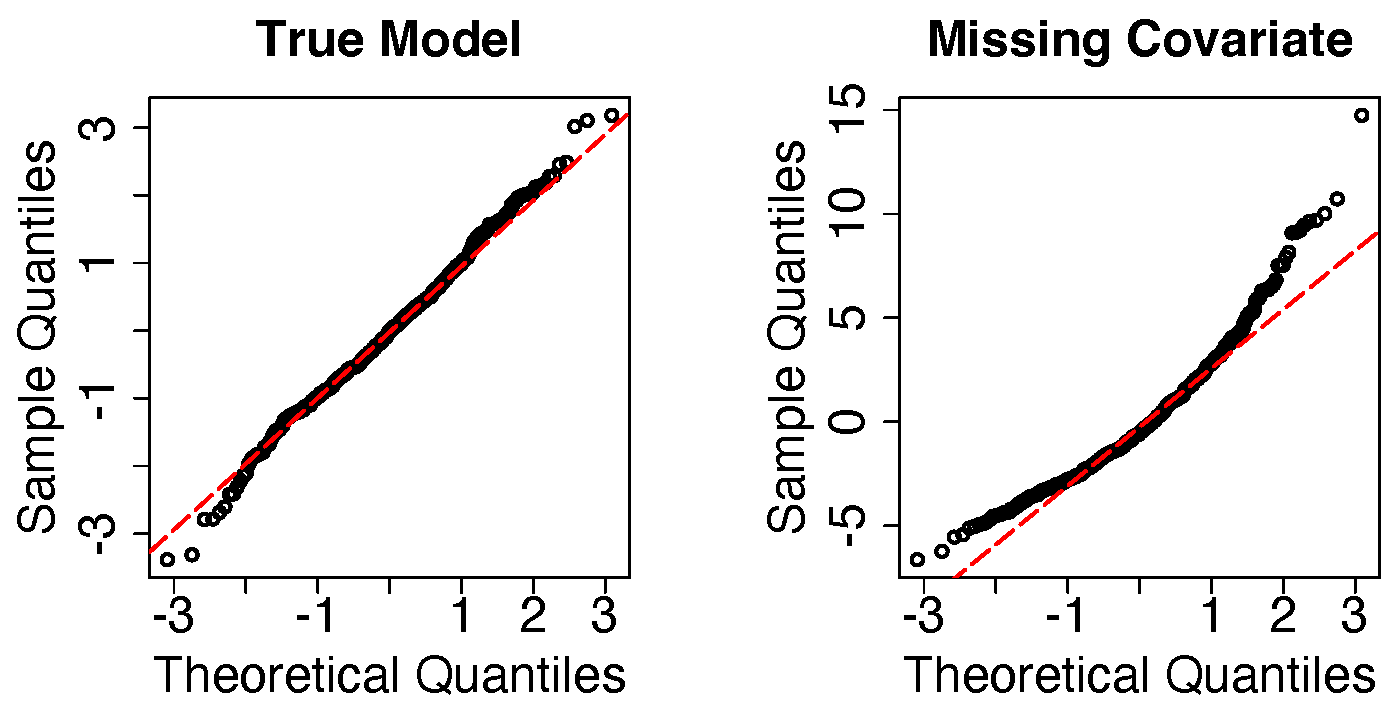
\includegraphics[width=0.8\textwidth]{figures/lmexam}
    \caption{QQ plots for linear regression model residuals.}
\end{figure}
\end{frame}

\begin{frame}{Residuals for linear regression models}
\protect\hypertarget{residuals-for-linear-regression-models-1}{}
\begin{itemize}
            \item Features of residuals  in linear regression models 
        \begin{itemize}
            \item Follow a known distribution under the correctly specified models
            \item Nearly identically distributed 
        \end{itemize}
        \vspace{0.1in}
    \item Graphical diagnostics: QQ plot, PP plot, residuals versus predictor plot
    \begin{itemize}
        \item Check normality assumption
        \item Identify other important factors
\item etc.
    \end{itemize}
    \vspace{0.1in}
    \item Construct overall goodness-of-fit tests using residuals

\end{itemize}
\end{frame}

\begin{frame}{Beyond Normality: Cox and Snell (1968)}
\protect\hypertarget{beyond-normality-cox1968general}{}
\begin{table}
\begin{tabular}{ccc}
    Linear Regression & &Generalization\\
\\
    $e_i =Y_i-X_i'\beta$&&$e_i=h(Y_i,X_i'\beta)$\\
    \\
                
                $e_i \sim N(0,\sigma^2)$ i.i.d &{\huge\textcolor{red}{$\Longrightarrow$}}&  $e_i$  i.i.d$\sim$known distribution \\
                \\
        $r_i=Y_i-X_i'\hat{\beta}$&&$R_i=h(Y_i,X_i'\hat{\beta})$\\
        \\
    $r_i$   are normally distributed &&$R_i$ follow a hypothesized pattern \\under the true model&&under the true model
\end{tabular}
\end{table}
\end{frame}

\begin{frame}{Residuals for Continuous Outcomes}
\protect\hypertarget{residuals-for-continuous-outcomes}{}
\begin{itemize}
    
    \item For \textcolor{blue}{continuous} variables $Y_i$, 
probability integral transform $F(Y_i|X_i,\beta)\sim \mathrm{Uniform}(0,1)$
\begin{itemize}
\item Gamma, inverse normal, lognormal distributions
\end{itemize}
\item Cox-Snell residuals  $F(Y_i|X_i,\hat{\beta}),i=1,\ldots,n$ should be uniform with correctly specified models
\end{itemize}
\vspace{-0.4in}
\begin{figure}[h]
\includegraphics[width=.8\textwidth]{figures/continuous}
\caption{Histogram and PP plot of Cox-Snell  residuals for a gamma example. }
\end{figure}
\end{frame}

\begin{frame}{Commonly Used Residuals for Discrete Outcomes}
\protect\hypertarget{commonly-used-residuals-for-discrete-outcomes}{}
\begin{itemize}
\item  \textcolor{red}{Discrete} $Y_i$ cannot be expressed as transformations of $X_i'\beta$  and i.i.d. errors so Cox-Snell residuals are not applicable

    \item Pearson and deviance residuals are \textcolor{red}{approximately} normal under a correctly specified model
\item How Good Is the Approximation?
\begin{itemize}
    
    \item A simulated example: Poisson GLM with log link
\end{itemize}
\end{itemize}
\vspace{-0.1in}
\begin{figure}[h]
\includegraphics[width=0.8\textwidth]{figures/poisson2coefslides2}
\caption{PP plots of residuals for a Poisson GLM  under the \textcolor{blue}{\textbf{true model}}.}
\end{figure}
\end{frame}

\begin{frame}{\(m\)-Asymptotics}
\protect\hypertarget{m-asymptotics}{}
\begin{itemize}
\tightlist
\item
  \(m\): the number of trials of binomial distributions, or the Poisson
  means, which controls the discreteness level \vspace{0.2in}
\item
  \(m\)-asymptotics: deviance residuals are normally distributed with a
  discrepancy term of order at least \(O_p(m^{-1/2})\) (Pierce and
  Schafer (1986)) \vspace{0.2in}
\item
  When \(m\) is small, deviance residuals and Pearson residuals could
  have a large discrepancy with the null pattern even under the true
  model, even with large \(n\)
\end{itemize}
\end{frame}

\begin{frame}{Randomized Quantile Residuals (Dunn and Smyth (1996))}
\protect\hypertarget{randomized-quantile-residuals-dunn1996randomized}{}
\begin{itemize}
    \item Idea: transform discrete integer-valued data into continuous data by adding noise
    \item Let $a_i = \hat{F}_i(Y_i-1)$ and $b_i = \hat{F}_i(Y_i)$, then the randomized quantile
    residual
    $$ \hat{e}_{Ri} = \Phi^{-1} (V_i),$$
    where $V_i$ is a uniform random variable on the interval $(a_i,b_i]$ independent of $Y_i$.
    \item Null pattern: normality
\end{itemize}
\end{frame}

\begin{frame}[fragile]{}
\protect\hypertarget{section-6}{}
\scriptsize

\begin{Shaded}
\begin{Highlighting}[]
\FunctionTok{par}\NormalTok{(}\AttributeTok{mfrow=}\FunctionTok{c}\NormalTok{(}\DecValTok{1}\NormalTok{,}\DecValTok{2}\NormalTok{))}
\FunctionTok{library}\NormalTok{(statmod)}
\NormalTok{resr }\OtherTok{\textless{}{-}} \FunctionTok{qresid}\NormalTok{(freqmodelBC)}
\FunctionTok{qqnorm}\NormalTok{(resr[}\SpecialCharTok{{-}}\FunctionTok{which}\NormalTok{(}\FunctionTok{is.infinite}\NormalTok{(resr))])}
\FunctionTok{qqline}\NormalTok{(resr[}\SpecialCharTok{{-}}\FunctionTok{which}\NormalTok{(}\FunctionTok{is.infinite}\NormalTok{(resr))])}

\NormalTok{resrnb }\OtherTok{\textless{}{-}} \FunctionTok{qresid}\NormalTok{(freqmodelBCnb)}
\FunctionTok{qqnorm}\NormalTok{(resrnb[}\SpecialCharTok{{-}}\FunctionTok{which}\NormalTok{(}\FunctionTok{is.infinite}\NormalTok{(resrnb))])}
\FunctionTok{qqline}\NormalTok{(resrnb[}\SpecialCharTok{{-}}\FunctionTok{which}\NormalTok{(}\FunctionTok{is.infinite}\NormalTok{(resrnb))])}
\end{Highlighting}
\end{Shaded}

\includegraphics{week8_p1_files/figure-beamer/unnamed-chunk-11-1.pdf}
\end{frame}

\begin{frame}{Drawbacks of Randomized Quantile Residuals}
\protect\hypertarget{drawbacks-of-randomized-quantile-residuals}{}
\begin{itemize}
    \item The procedure injects noise to the data
    \item The behavior of the residuals depend on the realization of the noise
\vspace{-0.2in}
    \begin{figure}[h]
    \includegraphics[width=0.8\textwidth]{figures/randomizeseeds}
    \caption{PP plot of randomized quantile  residuals of a Poisson GLM example with two different random seeds. }
\end{figure}
    \item Not sensitive to misspecification
\end{itemize}
\end{frame}

\begin{frame}{Quasi-empirical residual distribution function (Yang
(2021))}
\protect\hypertarget{quasi-empirical-residual-distribution-function-yang2021assessment}{}
\begin{itemize}
\item  The   Quasi-empirical residual distribution function is an alternative to empirical  distribution function of Cox-Snell residuals
\item    The   Quasi-empirical residual distribution function, $\hat{U}(\cdot)$,
                        should be close to the identity function under true model 
    \begin{figure}[h]
        \includegraphics[width=0.8\textwidth]{figures/quickexample}
        \vspace{-0.1in}
        \caption{$\hat{U}$ and deviance residuals for  a Poisson example under the true model. }
    \end{figure}

\end{itemize}
\end{frame}

\begin{frame}{Quasi-empirical residual distribution function}
\protect\hypertarget{quasi-empirical-residual-distribution-function}{}
\begin{itemize}
\tightlist
\item
  If \(Y\) is continuous, for any fixed value \(s \in (0, 1)\),
  \begin{align}\label{unic}
    \Pr(F(Y|\mathbf{X}=\mathbf{x})\leq s)=s.
  \end{align}
\item
  Conditioning on \(\mathbf{X}=\mathbf{x}\), \eqref{unic} holds for
  discrete \(Y\) if and only if \(s=F(k| \mathbf{x})\) for some integer
  \(k\), i.e., \(\Pr \left(Y\leq k| F(k| \mathbf{X})=s\right)=s\).
\item
  Yang (2021) proposed to use the subset of the data for which
  \(F(k| \mathbf{X})\approx s\) to estimate
  \(\Pr(Y\leq k| F(k| \mathbf{X})\approx s)\) instead
\end{itemize}
\end{frame}

\begin{frame}{}
\protect\hypertarget{section-7}{}
\begin{itemize}
\tightlist
\item
  Define the grid point \(F(k| \mathbf{x})\) closest to \(s\) as
  \(H( s;X,\beta)\)
\item
  A kernel function \(K(\cdot)\) to is used assign weights to the
  observations depending on the distance of \(s\) and
  \(H( s;X_{i},\beta)\), \(K((H( s;X_{i},\beta)-s)/h_n)\), \(h_n\) is
  the bandwidth

  \begin{figure}[h]
          \centering
          \includegraphics[width=0.6\textwidth]{figures/Kernels}
          \caption{Kernel Functions}
      \end{figure}
\end{itemize}
\end{frame}

\begin{frame}{}
\protect\hypertarget{section-8}{}
\begin{itemize}
        
        \item 
        Define the quasi-empirical residual distribution function
        \begin{align}
        \begin{split}\label{esti}
        \hat{U}(s)=\sum_{i=1}^{n}W_{ni}1( F(Y_{i}|\mathbf{X}_i,\bm{\beta})\leq H( s;X_{i},{\beta})),
        \end{split}
        \end{align}
        where 
        $$W_{ni}=\frac{K((H( s;X_{i},{\beta})-s)/h_n)}
        {\sum_{i=1}^{n}K((H( s;X_{i},{\beta})-s)/h_n)}$$
        \item Comparison of empirical residual distribution function with $\hat{U}(s)$ 
        
        \begin{table}
            
            \begin{tabular}{cl}
                Continuous&$ \sum_{i=1}^{n}\textcolor{BrickRed}{\frac{1}{n}}1(F(Y_{i}|X_{i},{\beta}) \leq \textcolor{blue}{s})$\\Discrete
                &$\sum_{i=1}^{n}\textcolor{BrickRed}{W_{ni}}1( F(Y_{i}|\mathbf{X}_i,\bm{\beta})\leq \textcolor{blue}{H( s;X_{i},{\beta})})$
            \end{tabular}
        \end{table}
            \end{itemize}
\end{frame}

\begin{frame}{Model Diagnostics for LGPIF}
\protect\hypertarget{model-diagnostics-for-lgpif}{}
\begin{figure}
        \centering
            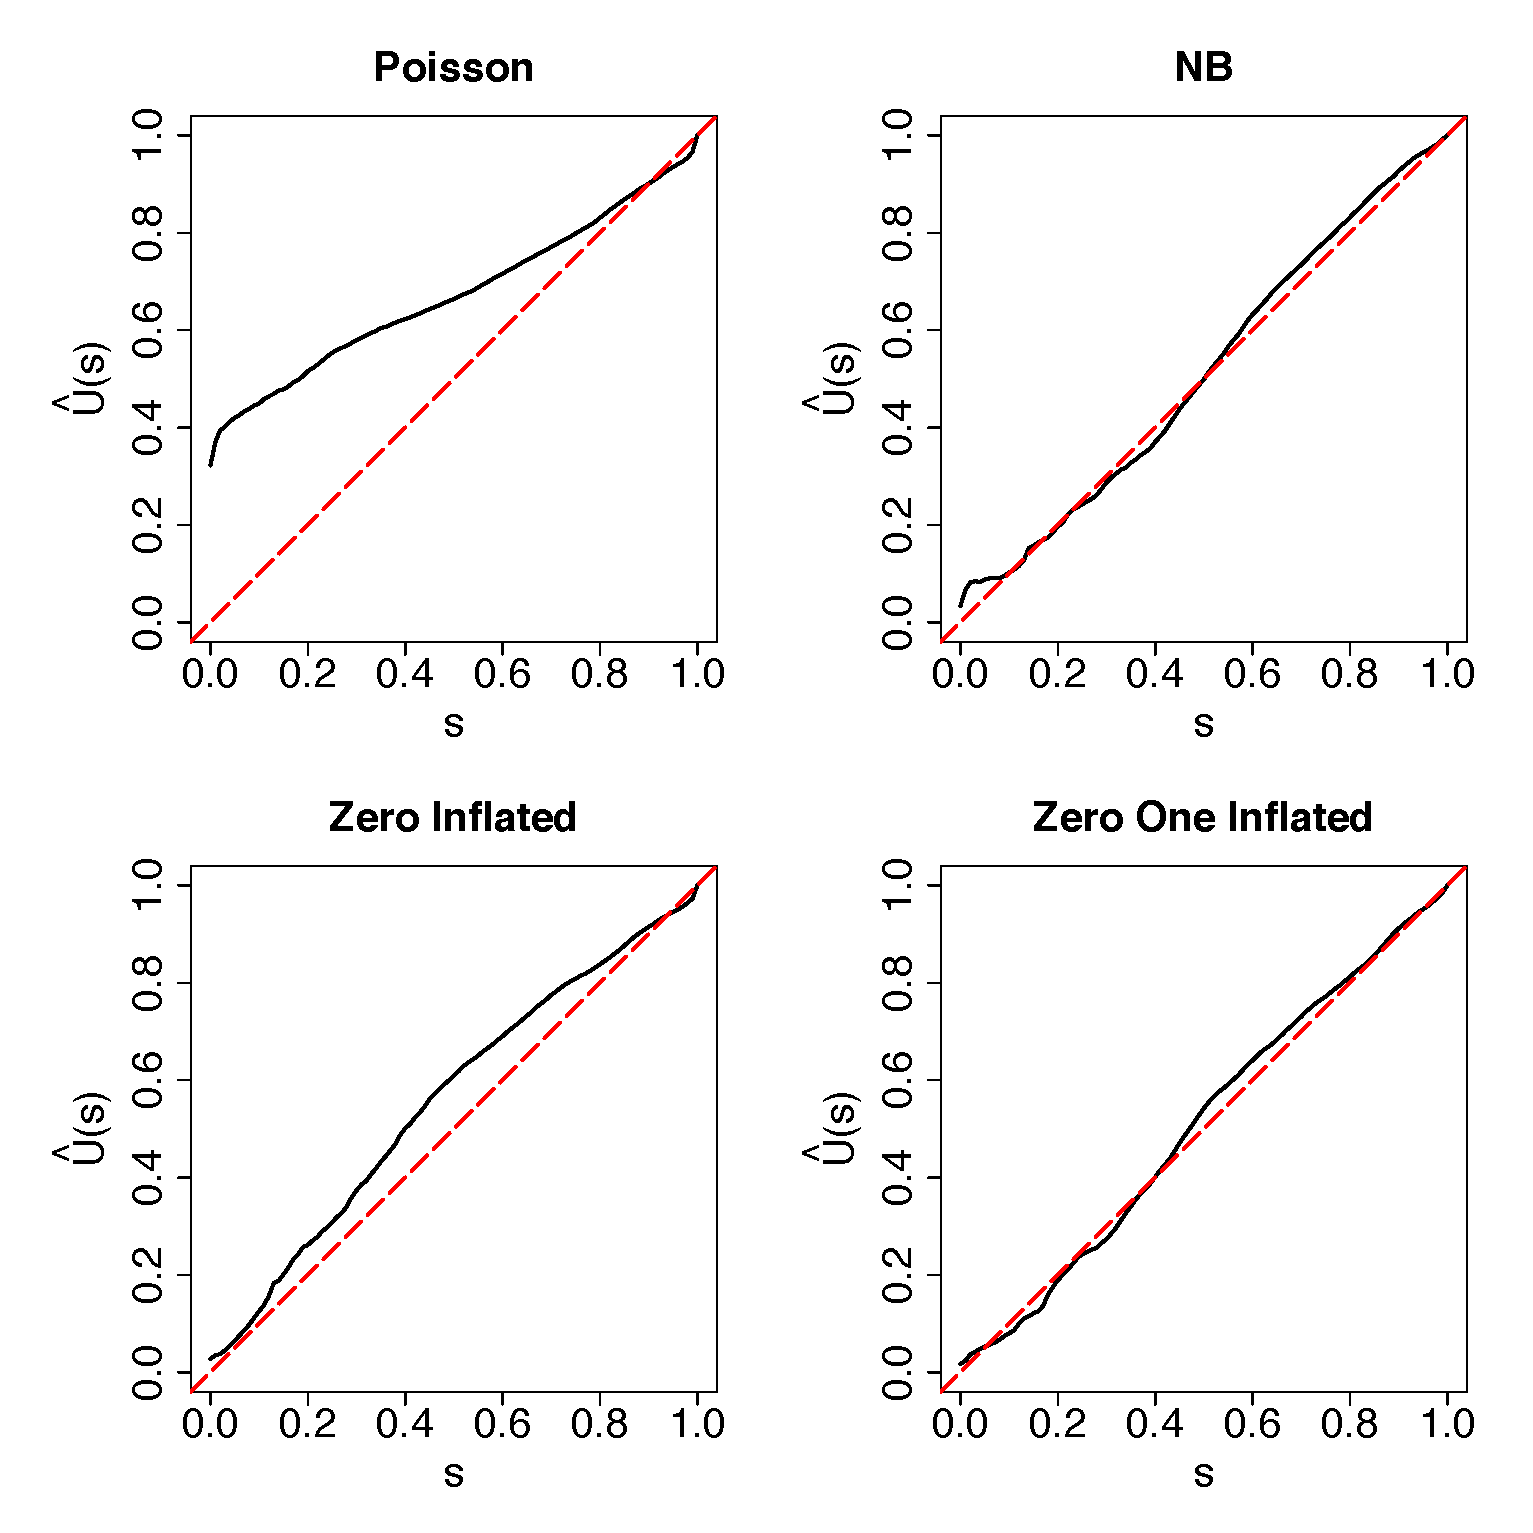
\includegraphics[width=.65\textwidth]{figures/marginplot}

        \caption{\small Plot of quasi-empirical residual distribution function $\hat{U}$ (Solid Line) for LGPIF data.}
\end{figure}
\end{frame}

\begin{frame}{Quasi-empirical residual distribution function}
\protect\hypertarget{quasi-empirical-residual-distribution-function-1}{}
\begin{itemize}
\tightlist
\item
  Pros

  \begin{itemize}
        \item is principled
            \item is close to the hypothesized pattern under the true model
            \item under the misspecified model, shows a significant discrepancy
        \end{itemize}
\item
  Cons

  \begin{itemize}
  \item does not produce residuals themselves and cannot identify causes of misspecification
  \item requires tuning bandwidth
  \item convergence rate $n^{-1/3}$
  \end{itemize}
\end{itemize}
\end{frame}

\begin{frame}{Double probability integral transform residuals (in
progress)}
\protect\hypertarget{double-probability-integral-transform-residuals-in-progress}{}
\begin{itemize}
\tightlist
\item
  \(F(Y|\mathbf{X})\) itself is not uniformly distributed for discrete
  outcomes
\item
  Another layer of probability integral transform,
  \(G_{0}\left(F(Y|\mathbf{X})\right)\), yields a uniform variable under
  the true model, where \(G_{0}\) is the distribution of
  \(F(Y|\mathbf{X})\)
\item
  The \textit{double probability integral transform residuals}
  \[  \hat{r}(Y_i|\mathbf{X}_i)=\hat{G}_{i}\left(F(Y_{i}|\mathbf{X}_i,\bm{\beta})\right)\]
  where \(\hat{G}_{i}\) is an estimator of \(G_{0}\) suited to the
  \(i\)th observation
  \[\hat{G}_{i}(s)=   \frac{1}{n-1}\sum_{j=1,j\neq i}^n {F}\left({F}^{(-1)}(s| \mathbf{X}_{j},\hat{\bm\beta})| \mathbf{X}_{j},\hat{\bm\beta}\right).\]
\end{itemize}
\end{frame}

\begin{frame}{Causes of misspecification}
\protect\hypertarget{causes-of-misspecification}{}
\begin{itemize}
\tightlist
\item
  Overdispersion: S-shaped pattern
\end{itemize}

\begin{figure}
    \centering
    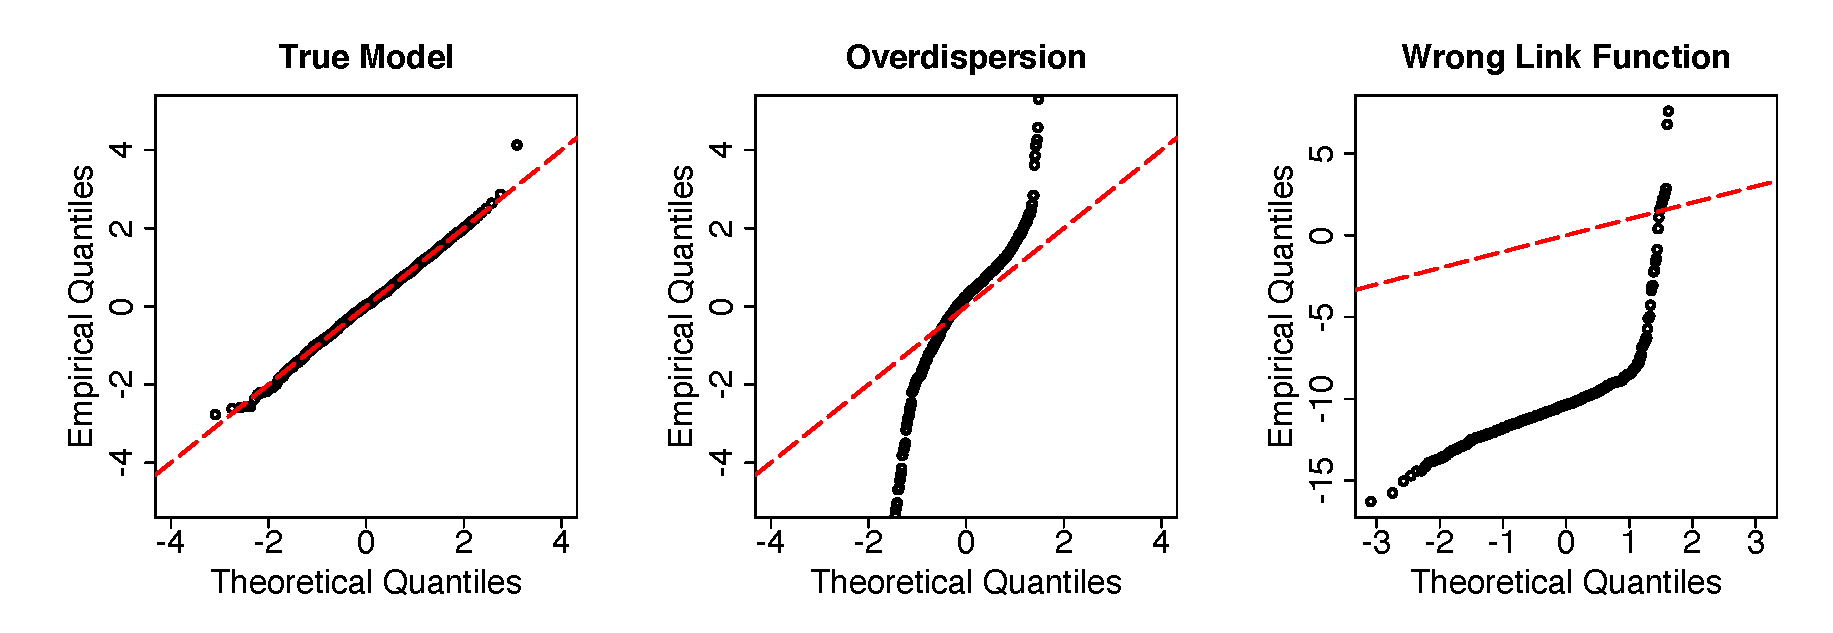
\includegraphics[width=\textwidth]{figures/othercause202111} 
\caption{QQ plots of the double  probability integral transform residuals under the correctly specified model (left) and models with overdispersion (middle) and an incorrect link function (right). \label{fig:other}}
\end{figure}
\end{frame}

\begin{frame}{References}
\protect\hypertarget{references}{}
\hypertarget{refs}{}
\begin{CSLReferences}{1}{0}
\leavevmode\vadjust pre{\hypertarget{ref-cox1968general}{}}%
Cox, David R, and E Joyce Snell. 1968. {``A General Definition of
Residuals.''} \emph{Journal of the Royal Statistical Society. Series B
(Methodological)}, 248--75.

\leavevmode\vadjust pre{\hypertarget{ref-dunn1996randomized}{}}%
Dunn, Peter K, and Gordon K Smyth. 1996. {``Randomized Quantile
Residuals.''} \emph{Journal of Computational and Graphical Statistics} 5
(3): 236--44.

\leavevmode\vadjust pre{\hypertarget{ref-pierce1986residuals}{}}%
Pierce, Donald A, and Daniel W Schafer. 1986. {``Residuals in
Generalized Linear Models.''} \emph{Journal of the American Statistical
Association} 81 (396): 977--86.

\leavevmode\vadjust pre{\hypertarget{ref-yang2021assessment}{}}%
Yang, Lu. 2021. {``Assessment of Regression Models with Discrete
Outcomes Using Quasi-Empirical Residual Distribution Functions.''}
\emph{Journal of Computational and Graphical Statistics} 30 (4):
1019--35.

\end{CSLReferences}
\end{frame}

\end{document}
